\documentclass[a4 paper]{article}
% Set target color model to RGB
\usepackage[inner=2.0cm,outer=2.0cm,top=2.5cm,bottom=2.5cm]{geometry}




\usepackage{setspace}
\usepackage[rgb]{xcolor}
\usepackage{verbatim}
\usepackage{subcaption}
\usepackage{amsgen,amsmath,amstext,amsbsy,amsopn,tikz,amssymb,tkz-linknodes}
\usepackage{fancyhdr}
\usepackage[colorlinks=true, urlcolor=blue,  linkcolor=blue, citecolor=blue]{hyperref}
\usepackage[colorinlistoftodos]{todonotes}
\usepackage{rotating}
\usepackage{listings}
%\usetikzlibrary{through,backgrounds}
\hypersetup{%
pdfauthor={Ashudeep Singh},%
pdftitle={Homework},%
pdfkeywords={Tikz,latex,bootstrap,uncertaintes},%
pdfcreator={PDFLaTeX},%
pdfproducer={PDFLaTeX},%
}


\usepackage{lettrine}
\usepackage{rotating}
\usepackage{lmodern}
\usepackage{dirtree}
\usepackage{placeins}
\usepackage{listings}
\lstset{
	basicstyle=\footnotesize\ttfamily,
	columns=flexible,
	breaklines=true,
	numbers=left,
	%stepsize=1,
	numberstyle=\tiny,
	backgroundcolor=\color[rgb]{0.85,0.90,1}
}

\lstnewenvironment{lstlistingbash}{\lstset{basicstyle=\footnotesize\ttfamily,
		columns=flexible,
		breaklines=true,
		numbers=left,
		%stepsize=1,
		numberstyle=\tiny,
		backgroundcolor=\color[rgb]{1,0,.4}}}{}


\lstnewenvironment{lstlistingoutput}{\lstset{basicstyle=\footnotesize\ttfamily,
		columns=flexible,
		breaklines=true,
		numbers=left,
		%stepsize=1,
		numberstyle=\tiny,
		backgroundcolor=\color[rgb]{.7,.7,.7}}}{}



\let\oldquote\quote
\let\endoldquote\endquote
\renewenvironment{quote}{
	\oldquote\footnotesize
	\lettrine[lines=3]{\color{BrickRed}!}{ }}
{\endoldquote}

\newenvironment{question}{
	\oldquote\footnotesize
	\lettrine[lines=3]{\color{BrickRed}?}{ }}
{\endoldquote}


%\usetikzlibrary{shadows}
% \usepackage[francais]{babel}
\usepackage{booktabs}
\newcommand{\ra}[1]{\renewcommand{\arraystretch}{#1}}

\newtheorem{thm}{Theorem}[section]
\newtheorem{prop}[thm]{Proposition}
\newtheorem{lem}[thm]{Lemma}
\newtheorem{cor}[thm]{Corollary}
\newtheorem{defn}[thm]{Definition}
\newtheorem{rem}[thm]{Remark}
\numberwithin{equation}{section}

\newcommand{\homework}[6]{
   \pagestyle{myheadings}
   \thispagestyle{plain}
   \newpage
   \setcounter{page}{1}
   \noindent
   \begin{center}
   \framebox{
      \vbox{\vspace{2mm}
    \hbox to 6.28in { {\bf Gesis:~A Practical Introduction to Machine Learning in Python\hfill {\small }} }
       \vspace{6mm}
       \hbox to 6.28in { {\Large \hfill #1  \hfill} }
       \vspace{6mm}
   
       %\hbox to 6.28in { {\it TA: #4  \hfill #6}}
      \vspace{2mm}}
   }
   \end{center}
   \markboth{#5 -- #1}{#5 -- #1}
   \vspace*{4mm}
}

\newcommand{\problem}[2]{~\\\fbox{\textbf{Problem #1}}\hfill (#2 points)\newline\newline}
\newcommand{\subproblem}[1]{~\newline\textbf{(#1)}}
\newcommand{\D}{\mathcal{D}}
\newcommand{\Hy}{\mathcal{H}}
\newcommand{\VS}{\textrm{VS}}
\newcommand{\solution}{~\newline\textbf{\textit{(Solution)}} }

\newcommand{\bbF}{\mathbb{F}}
\newcommand{\bbX}{\mathbb{X}}
\newcommand{\bI}{\mathbf{I}}
\newcommand{\bX}{\mathbf{X}}
\newcommand{\bY}{\mathbf{Y}}
\newcommand{\bepsilon}{\boldsymbol{\epsilon}}
\newcommand{\balpha}{\boldsymbol{\alpha}}
\newcommand{\bbeta}{\boldsymbol{\beta}}
\newcommand{\0}{\mathbf{0}}


\begin{document}
\homework{Exercise: Describing an existing structured dataset}{}{}{}{}{}

\section{Downloading the data}
In this exercise, you will do some basic descriptive analyses of an existing dataset. Mazieres (2014) scraped data from online porn sites, resulting in two datasets with  metadata about almost two million amateur porn videos. We will work with one of these datasets, consisting of all metadata on all videos posted on \url{http://xhamster.com} from its creation in 2007 until February 2013. The authors made the dataset available on on \url{http://sexualitics.github.io}, and you can find a description of it in Figure~\ref{fig:sexualitics}.

\begin{figure}[h!]
\centering
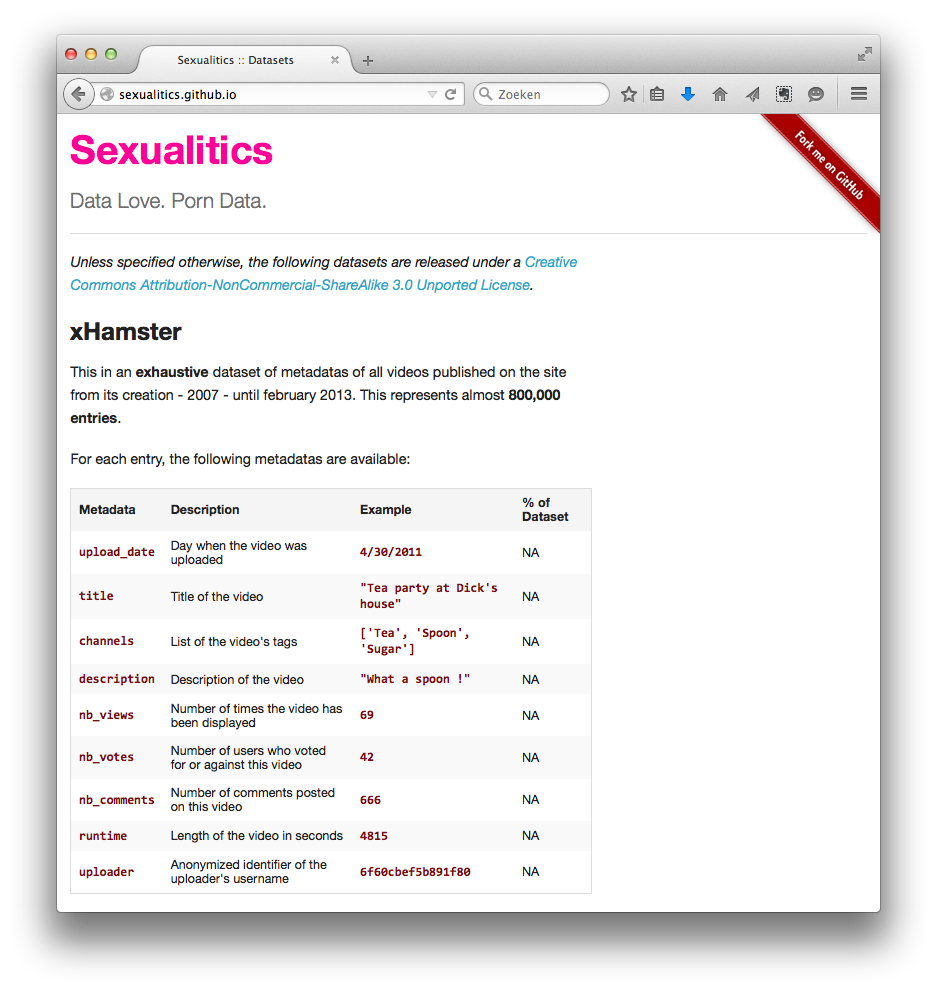
\includegraphics[width=.75\paperwidth,keepaspectratio]{../pictures/sexualitics.png}
\caption{\label{fig:sexualitics}The discription of the dataset.}
\end{figure}

We do the exercise together in class, but make sure you have downloaded the dataset before class. You can do so as follows (but, of course, replace ``damian'' with your own user name):
\begin{lstlistingbash}
cd /home/damian
mkdir pornexercise
cd pornexercise
wget pornstudies.sexualitics.org/data/xhamster.json.tar.gz
tar -xzf xhamster.json.tar.gz
\end{lstlistingbash}
The \texttt{wget} command downloads the dataset. It is compressed, so we have to uncompress it, which is done by the \texttt{tar} command (most of you probably are used to having \texttt{.zip} files for compressed or archived data, which is essentially the same; \texttt{.tar.gz} is more common among the nerdier part of the population).
Lets check if everything went right:
\begin{lstlistingbash}
ls -lh
\end{lstlistingbash}
should give you an output like this:
\begin{lstlistingoutput}
damian@damian-VirtualBox:~/pornexercise\$ ls -lh
total 284M
-rw-r--r-- 1 damian damian 229M feb  8  2014 xhamster.json
-rw-rw-r-- 1 damian damian  55M feb  8  2014 xhamster.json.tar.gz
\end{lstlistingoutput}
You see that the compressed file is 55MB large, but the uncompressed one is more than four times as large. Let's delete the compressed one, we don't need it any more:
\begin{lstlistingbash}
rm xhamster.json.tar.gz
\end{lstlistingbash}



\section{The tasks}
Start with having a look at Figure~\ref{fig:sexualitics}. It is important to understand the structure of the data: Which fields are there, how are they named, and what do they contain? For example, we see that the field ``channels'' contains a \emph{list} of different tags, while ``nb\_votes'' seems to contain an \emph{integer}.
Ready to go? Let's do some work:

\begin{enumerate}
\item Print the title of each video.
\item
	\begin{enumerate} 
	 \item What are the 100 most frequently used tags?
	 \item What is the average number of tags per video?
	\end{enumerate}
\item What tags generate the most comments/votes/views?
\item What is the average length of a video description?
\item What are the most frequently used words in the descriptions?
\item Write a short script to train a Naive Bayes classifier on the dataset. Specifically, train a model that will classify a specific video description according to the level of responses it will elicit: low (i.e., less than 25 comments) or high (i.e.  25 or more comments). 
\end{enumerate}


\section{Hints}
The following hints will help you solving the exercise.

\subsection*{Task 1}

You haven't learned yet how to handle JSON-files. This is explained in chapter 4 in detail. For now, you only have to know that you can read the data into a Python dict with the following command:

\begin{lstlisting}
import json
with open (`/home/damian/WHATEVERTHEFILEISCALLED.json') as f:
    data=json.load(f)
\end{lstlisting}

You now have a dict called data. This is, however, a very large dataset. To practice and play around with the data, you might want to consider taking a random sample: 

\begin{lstlisting}
data_short = dict(random.sample(data.items(), 100) )
\end{lstlisting}


This dict consists of other dicts, each of which contains information on one video clip. We can loop over the keys and values of the outer dict to get the data we want:

\begin{lstlisting}
for key, value in data.items():
   print(value["title"])
\end{lstlisting}

You could print the key as well (try it!), if you are interested in the number of the clip to which the title belongs.

You know from Figure~\ref{fig:sexualitics} that the key we are interested in is called "title".

That's it!


\subsection*{Task 2}

There is a module called Counter that allows you to count elements in a list.

Consister this example to print the two most frequent words in a list:

\begin{lstlisting}
from collections import Counter

l = ['hi','hi','hi','bye','bye','hi','doei','hoi']
c = Counter(l)
print(c.most_common(2))
\end{lstlisting}

This gives as a result: 

\begin{lstlistingoutput}
[('hi', 4), ('bye', 2)]
\end{lstlistingoutput}


To solve this task, you probably want to create an empty list for the tags first, and then loop over your data to fill the list. After you have this list, you can use a counter to determine the frequencies. 


\begin{quote}
If you do this on \emph{really} big datasets, there is a replacement for Counter called bounter, see \url{https://github.com/RaRe-Technologies/bounter}
\end{quote}


\subsection*{Task 3}

You might want to construct a dict with the categories as keys and an int containing the number of comments. Then you loop over your dataset and each time you encounter the same category, you add the number of comments to the dictionary entry. However, the first time you encounter a category, it does not have a key yet. We can use a so-called defaultdict, that just returns a default value (\texttt{0} for an int, \texttt{""} for a string,\ldots) if it isn't there yet. 

\begin{lstlisting}
from collections import defaultdict
commentspercat=defaultdict(int)
\end{lstlisting}
And then, loop over the dataset and add \texttt{int(value["nb\_comments"])} to the dict.

Not all items might have comments and have a value of 'NA' instead. Thus, referring to \texttt{int(data[item]["nb\_comments"])} might fail. You can specify what should happen in such cases by using a try-except construction:

\begin{lstlisting}
try:
    commentspercat[category]+=int(value['nb_comments'])
except: 
    pass
\end{lstlisting}

This just means that if the line fails, it just continues without any error message.



\subsection*{Task 4}
This is basically the same what you've already done...


\subsection*{Task 5}
You can transform a string to a list of words by using the split method.
\begin{lstlisting}
"this is a test".split()
\end{lstlisting}
results in
\begin{lstlistingoutput}
["this", "is", "a", "test"]
\end{lstlistingoutput}
(useful for applying a Counter...)

\subsection*{Task 6}
Start by composing a list that assigns the number 1 to videos receiving 25 comments or more, and 0 to videos receiving less than 25 comments. Consider how you want to handle missing data ("NA"). If you want to remove these cases, consider the following example. 
\begin{lstlisting}
comments = [v['nb_comments'] for k, v in data.items() if v['nb_comments'] != "NA"]
\end{lstlisting}


On the next page, you will find the solution.

\newpage
\section{Solution}
Try first to do it yourself, but if you cannot find out how to do it, you can have a look at the example solution below.

\begin{lstlisting}
import json
from collections import Counter
from collections import defaultdict

#Right path?
with open(`/home/damian/pornexercise/xhamster.json') as fi:
    data=json.load(fi)


#%% task 1: print titles
for k,v in data.items():
    print (v["title"])



#%% task 2a en 2b: average tags per video and most frequently used tags

alltags=[]
i=0
for identifyer,clip in data.items():
    i+=1
    alltags.extend(clip["channels"])

print(len(alltags),"tags have been used to describe the",i,"different videos")
print("Thus, we have an average of",len(alltags)/i,"tags per video")
c=Counter(alltags)
print (c.most_common(100))



#%% task 3: What porn category is most frequently commented on?
commentspercat=defaultdict(int)
for identifier,clip in data.items():
    for tag in clip["channels"]:
        try:
            commentspercat[tag]+=int(clip["nb_comments"])
        except:
            pass

print(commentspercat)

# or nicer:
for tag in sorted(commentspercat, key=commentspercat.get, reverse=True):
    print(tag, commentspercat[tag])



#%%task 4: average length of text 
length=[]
for identifier,clip in data.items():
    length.append(len(clip["description"]))

print ('Average length',sum(length)/len(length))


#%%task 5:  most frequently used words

# most frequently used words
allwords=[]
for identifier,clip in data.items():
    allwords.extend(clip["description"].split())
c2=Counter(allwords)
print(c2.most_common(100))


#%%task 6:  classification


from sklearn.model_selection import train_test_split
from sklearn.naive_bayes import MultinomialNB
from sklearn.feature_extraction.text import CountVectorizer
from sklearn.metrics import confusion_matrix, classification_report


comments = [v[`nb_comments'] for k, v in data.items() if v[`nb_comments'] != "NA"]
description = [v[`description'] for k, v in data.items() if v[`nb_comments'] != "NA"]
responsive = [0 if i < 25 else 1 for i in comments]


X_train, X_test, y_train, y_test = train_test_split(description, responsive, test_size = 0.2 , random_state=42)

vectorizer = CountVectorizer(stop_words='english')
X_train = vectorizer.fit_transform(X_train)
X_test = vectorizer.transform(X_test)

nb = MultinomialNB()
nb.fit(X_train, y_train)

y_pred = nb.predict(X_test)

print(confusion_matrix(y_test, y_pred))
print(classification_report(y_test, y_pred))

\end{lstlisting}




\end{document} 
